\documentclass[10pt,a4paper]{amsart}
\usepackage{amsmath,amssymb,amsthm,graphicx}
\usepackage{amsmath,amssymb,graphicx,xcolor,mathtools}
\providecommand{\invamp}{\mathbin{\rotatebox[origin=c]{180}{\&}}}
\providecommand{\wn}{\mathord{?}}
\title{Sequentialization of DR-correct multiplicative proof structures with mix}
\author{Rémi Di Guardia, Olivier Laurent, Lorenzo Tortora de Falco, Lionel Vaux Auclair}
\date{doi:10.4230/LIPIcs.FSCD.2025.16; CC BY 4.0}
\begin{document}
\maketitle
\noindent\textit{Editorial note.} Source: https://drops.dagstuhl.de/entities/document/10.4230/LIPIcs.FSCD.2025.16. © the four authors, CC BY 4.0. Editable text transcribed from the official HTML; graph and inference-rule artwork retained from publisher SVG.\par\medskip
\noindent\textit{Allowed standard prerequisites (editorial).}\begin{itemize}
\item Finite partial graph paths and elementary ordering facts. Author §2 and §3 definitions; Lemmas4/5 are stated without separate proof in the publication and retained unchanged.
\end{itemize}\medskip
% BEGIN S2
 
\par\medskip\noindent\textbf{2 Graphs and Cusps}\par
 
% BEGIN S2.SS1
 
\par\medskip\noindent\textbf{2.1 Partial Undirected Graphs and Paths}\par
 
% BEGIN S2.SS1.p1
 
As we take interest in proof nets and Yeo’s theorem in this paper, we study undirected paths in finite undirected partial multigraphs. We recall here quickly some basic notions from graph theory, for more details we refer the reader to [2].\par
 
% END S2.SS1.p1
 
% BEGIN S2.SS1.p2
 
A (finite undirected multi) partial graph (without loop) is a triple $(\mathcal{V},\mathcal{E},\psi)$ where $\mathcal{V}$ (vertices) and $\mathcal{E}$ (edges) are finite sets and $\psi$ (the incidence function) associates to each edge a set of at most two vertices. An edge $e$ is total when $\psi(e)$ is of cardinal two, and a total graph (or simply a graph) is one whose edges are total. Many notions lift immediately from total graphs to partial graphs, e.g. isomorphisms – that we denote $\simeq$. An edge $e$ is incident to a vertex $v$ if $v\in\psi(e)$, in which case $v$ is an endpoint of $e$.\par
 
% END S2.SS1.p2
 
% BEGIN S2.SS1.p3
 
A path $p$ is a finite alternating sequence of vertices and edges $(v_{0},e_{1},v_{1},e_{2},v_{2},\dots,e_{n},v_{n})$ such that for all $i\in\{1;\dots;n\}$, the endpoints of $e_{i}$ are exactly $v_{i-1}$ and $v_{i}$ (which are distinct). A path always has at least one vertex, but it can have no edge and be reduced to a single vertex $(v_{0})$, in which case it is called an empty path. With the notation above, $v_{0}$ is the source of $p$, $v_{n}$ is its target and both make the endpoints of $p$. Since a given vertex may occur more than once in a path, we may have to talk about occurrences of vertices in a path to distinguish these equal values. We use the following notations:\par
  
\par\noindent  $\blacksquare$ 
% BEGIN S2.I1.i1.p1
 
the concatenation of two paths $p_{1}=(v_{0},e_{1},\dots,e_{k},v_{k})$ and $p_{2}=(v_{k},e_{k+1},\dots,e_{n},v_{n})$ is the path $p_{1}\cdot p_{2}=(v_{0},e_{1},\dots,e_{k},v_{k},e_{k+1},\dots,e_{n},v_{n})$;\par
 
% END S2.I1.i1.p1
 
 
\par\noindent  $\blacksquare$ 
% BEGIN S2.I1.i2.p1
 
the reverse of a path $p=(v_{0},e_{1},v_{1},\dots,e_{k},v_{k})$ is $\overline{p}=(v_{k},e_{k},v_{k-1},\dots,e_{1},v_{0})$;\par
 
% END S2.I1.i2.p1
 
 
\par\noindent  $\blacksquare$ 
% BEGIN S2.I1.i3.p1
 
if $v$ and $u$ are two (occurrences of) vertices of a path $p$, with $v$ occurring before $u$, ${p}_{(v,u)}$ is the unique sub-path (i.e. sub-sequence that is a path) of $p$ with source $v$ and target $u$.\par
 
% END S2.I1.i3.p1
 
  
% END S2.SS1.p3
 
% BEGIN S2.SS1.p4
 
A path is simple if its edges are pairwise distinct and its vertices are pairwise distinct except possibly its endpoints which may be equal. A path is closed if it has equal endpoints, otherwise it is open. A cycle is a non-empty simple closed path.\par
 
% END S2.SS1.p4
 
% BEGIN S2.SS1.p5
 
Given a partial graph $G=(\mathcal{V},\mathcal{E},\psi)$, a sub-graph of $G$ is a partial graph $G^{\prime}=(\mathcal{V}^{\prime},\mathcal{E}^{\prime},\psi^{\prime})$ such that $\mathcal{V}^{\prime}\subseteq\mathcal{V}$, $\mathcal{E}^{\prime}\subseteq\mathcal{E}$ and $\psi^{\prime}$ is the restriction of $\psi$ to $\mathcal{E}^{\prime}$ in its domain and sets of $\mathcal{V}^{\prime}$ in its codomain. Connectedness is not immediate to define in partial graphs because paths go from vertices to vertices. Two vertices $v$ and $u$ are connected when there exists a path with endpoints $v$ and $u$. Two edges are connected if they are incident to two connected vertices. An edge $e$ and a vertex $v$ are connected if $e$ is incident to a vertex connected to $v$. A partial graph $G$ is connected when any two different vertices or edges of $G$ are connected. A connected component is a non-empty connected sub-graph maximal for the inclusion.\par
 
% END S2.SS1.p5
 
% END S2.SS1
 
% BEGIN S2.SS2
 
\par\medskip\noindent\textbf{2.2 Local Coloring and Cusps}\par
 
% BEGIN S2.SS2.p1
 
Let $G$ be a (partial) graph. A local coloring of $G$ is a function c taking as arguments an edge $e$ and one of its endpoints $v$. By convention, the elements $\textnormal{{c}}(e,v)$ are called colors. The intuition is that given an edge $e$ and one of its endpoints $v$, $\textnormal{{c}}(e,v)$ is the color of $e$ according to $v$. A local coloring can also be seen as a coloring of half-edges, i.e. $\textnormal{{c}}(e,v)$ is the color of the half of $e$ near $v$. When drawing a graph, we therefore represent $\textnormal{{c}}(e,v)$ by coloring the part of $e$ touching $v$, with colors also given by the shape of the edges (solid, dashed, …). We recover the standard notion of edge-coloring, which maps edges to colors, when for every edge $e$, $\textnormal{{c}}(e,\_)$ has the same value for all endpoints of $e$. An example of locally colored graph is given on Figure 3, where $\textnormal{{c}}(e,v)=\text{{\color[rgb]{1,0,0}\definecolor[named]{%
pgfstrokecolor}{rgb}{1,0,0}solid}}$, $\textnormal{{c}}(e,u)=\text{{\color[rgb]{1,0,0}\definecolor[named]{%
pgfstrokecolor}{rgb}{1,0,0}solid}}$, $\textnormal{{c}}(f,u)=\text{{\color[rgb]{1,0,0}\definecolor[named]{%
pgfstrokecolor}{rgb}{1,0,0}solid}}$, $\textnormal{{c}}(f,w)=\text{{\color[rgb]{0,0,1}\definecolor[named]{%
pgfstrokecolor}{rgb}{0,0,1}dashed}}$, $\textnormal{{c}}(g,v)=\text{{\color[rgb]{0,0,1}\definecolor[named]{%
pgfstrokecolor}{rgb}{0,0,1}dashed}}$, $\textnormal{{c}}(g,w)=\text{{\color[rgb]{1,0,0}\definecolor[named]{%
pgfstrokecolor}{rgb}{1,0,0}solid}}$ and $\textnormal{{c}}(h,v)=\text{{\color[rgb]{.5,0,.5}\definecolor[named]{%
pgfstrokecolor}{rgb}{.5,0,.5}dotted}}$.\par
 
% END S2.SS2.p1
 
% BEGIN S2.SS2.p2
 
A cusp at $v$ of color $\alpha$ is a triple $(e,v,f)$ where $e$ and $f$ are distinct edges such that $v$ is an endpoint of both of these edges and $\textnormal{{c}}(e,v)=\alpha=\textnormal{{c}}(f,v)$. In this case, $v$ is called the vertex of the cusp, $\alpha$ the color of the cusp and $(v,\alpha)$ is called a cusp-point. More generally, we will consider in this paper vertex-color pairs which are pairs made of a vertex and a color, and a cusp-point is a particular instance of a vertex-color pair. The locally colored graph in Figure 3 has two cusps, $(e,u,f)$ and $(f,u,e)$, both of vertex $u$ and color solid, so that $(u,\text{{\color[rgb]{1,0,0}\definecolor[named]{pgfstrokecolor}{rgb}{1,0,0}%
solid}})$ is the only cusp-point of this graph.\par
 
% END S2.SS2.p2
 
% BEGIN S2.SS2.p3
 
A cusp of a path $p$ is a cusp made by a sub-sequence $(e,v,f)$ of this path or, in case $p$ is closed, a cusp $(e_{n},v_{0},e_{1})$ made by its last edge $e_{n}$, its source (and target) $v_{0}$ and its first edge $e_{1}$. Remark that the reverse of a path contains the same number of cusps as this path. A cusp-free path, also called an alternating path, is one without cusp. Given a non-empty path $p$, whose source is $v_{0}$ and first edge is $e_{1}$, its starting color is $\textnormal{{c}}(e_{1},v_{0})$. Similarly, if its target is $v_{n}$ and its last edge is $e_{n}$, then the ending color of $p$ is $\textnormal{{c}}(e_{n},v_{n})$. Remark the starting (resp. ending) color of $\overline{p}$ is the ending (resp. starting) color of $p$. For instance, in the graph depicted on Figure 3 the path $(v,e,u,f,w)$ has one cusp at $u$ of color solid, its starting color is solid and its ending one is dashed.\par
 
% END S2.SS2.p3
 
% BEGIN Thmtheorem1
 
\par\medskip\noindent\textbf{Fact 1.}\par
 
% BEGIN Thmtheorem1.p1
 
Let $\omega$ be a cycle with no cusp at its source, and $\alpha$ a color. Then $\alpha$ is not the starting color of $\omega$ or $\alpha$ is not the starting color of $\overline{\omega}$.\par
 
% END Thmtheorem1.p1
 
% END Thmtheorem1
 
% BEGIN S2.SS2.p4
 
We call splitting a vertex $v$ such that any cycle containing it has a cusp at $v$. We will show in Section 6.1 that this fits the notion at play in the conclusion of Yeo’s theorem [39].\par
 
% END S2.SS2.p4
 
% BEGIN Thmtheorem2
 
\par\medskip\noindent\textbf{$\blacktriangleright$ Remark 2.}\par
 
% BEGIN Thmtheorem2.p1
 
We invented this “local coloring”, which is not standard in the literature, and the name “cusp”. When used only through the notions of cusps and splitting vertices, that a given color is used on different vertices has no impact. Hence, we could use different sets of colors depending on each vertex, or not use more colors than the maximal degree of the graph. Equivalently, a local coloring is an equivalence relation on the edges incident to $v$, for each vertex $v$. We keep the idea of local coloring as it is a direct generalization of edge-coloring.\par
 
% END Thmtheorem2.p1
 
% END Thmtheorem2
 
% BEGIN S2.F3
   
% BEGIN S2.F3.fig1

\begin{center}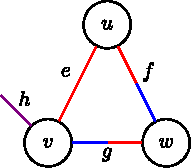
\includegraphics[width=0.75\linewidth,height=0.4\textheight,keepaspectratio]{graphic-01.pdf}\end{center}
 
Figure 2: Example of locally colored graph.\par
 
% END S2.F3.fig1
   
% BEGIN S2.F3.fig2
 
\begin{center}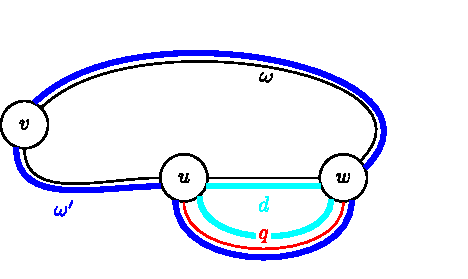
\includegraphics[width=0.75\linewidth,height=0.4\textheight,keepaspectratio]{graphic-02.pdf}\end{center}\par
 
Figure 3: Illustration of Lemma 6.\par
 
% END S2.F3.fig2
   
% END S2.F3
 
% END S2.SS2
 
% END S2


% BEGIN S3
 
\par\medskip\noindent\textbf{3 A Generalization of Yeo’s Theorem}\par
 
% BEGIN S3.p1
 
We prove a version of Yeo’s theorem [39] for locally colored partial graphs, which is moreover parametrized by the choice of a set of vertex-color pairs (subject to a technical condition): Theorem 8. We first fix a partial graph $G$ with a local coloring c.\par
 
% END S3.p1
 
% BEGIN S3.p2
 
The main idea is to follow a path that is an evidence of progression, i.e. a strict partial order $\Rsh$: a vertex is smaller than another when there is a path from the first to the second, and we will prove that a maximal vertex is splitting. As the hypothesis of the theorem is about cusp-free cycles, it makes sense to consider cusp-free paths in this ordering. However, two issues prevent $\Rsh$ from being an order. First, the concatenation of two cusp-free paths may not be cusp-free. To have $\Rsh$ transitive, we impose a condition on the starting and ending colors of the cusp-free path – which is why we consider vertex-color pairs and not simply vertices. Second, there is no reason for this relation $\Rsh$ of “being linked by a cusp-free path” to not loop. Hence, we add a condition on the path that there is no way to go back on it, yielding from $\Rsh$ a relation $\lhd$ which will be our strict partial order. This entails the following:\par
 
% END S3.p2
 
% BEGIN Thmtheorem3
 
\par\medskip\noindent\textbf{Definition 3.}\par
 
% BEGIN Thmtheorem3.p1
 
Given vertices $v$ and $u$, and colors $\alpha$ and $\beta$, we write $(v,\alpha)\overset{p}{\Rsh}(u,\beta)$ if $p$ is a simple open cusp-free path from $v$ to $u$ with starting color not $\alpha$ and with ending color $\beta$. We note $(v,\alpha)\overset{p}{\lhd}(u,\beta)$ when $(v,\alpha)\overset{p}{\Rsh}(u,\beta)$ and for all vertex $w$, color $\tau$ and path $q$ such that $(u,\beta)\overset{q}{\Rsh}(w,\tau)$, $w$ is not in $p$. We simply write $(v,\alpha)\lhd(u,\beta)$ when such a path exists.\par
 
% END Thmtheorem3.p1
 
% END Thmtheorem3
 
% BEGIN Thmtheorem4
 
\par\medskip\noindent\textbf{Lemma 4.}\par
 
% BEGIN Thmtheorem4.p1
 
Let $v$, $u$ and $w$ be vertices, $\alpha$, $\beta$ and $\tau$ be colors, and $p$ and $q$ be paths. If $(v,\alpha)\overset{p}{\lhd}(u,\beta)$ and $(u,\beta)\overset{q}{\Rsh}(w,\tau)$ then $(v,\alpha)\overset{p\cdot q}{\Rsh}(w,\tau)$.\par
 
% END Thmtheorem4.p1
 
% END Thmtheorem4
 
% BEGIN Thmtheorem5
 
\par\medskip\noindent\textbf{Lemma 5.}\par
 
% BEGIN Thmtheorem5.p1
 
The relation $\lhd$ is a strict partial order on vertex-color pairs.\par
 
% END Thmtheorem5.p1
 
% END Thmtheorem5
 
% BEGIN S3.p3
 
The key ingredient for proving our Yeo-style theorem is showing that for any pair $(v,\alpha)$ maximal for the strict partial order $\lhd$, $v$ is splitting. It is a consequence of the following:\par
 
% END S3.p3
 
% BEGIN Thmtheorem6
 
\par\medskip\noindent\textbf{Lemma 6 (Cusp Minimization).}\par
 
% BEGIN Thmtheorem6.p1
 
Fix a partial graph $G$ with a local coloring. Assume $\omega$ is a cycle starting from a vertex $v$, with no cusp at $v$ but containing a cusp of vertex $u$ and color $\alpha$. If $(u,\alpha)\overset{q}{\Rsh}(w,\beta)$ with $w$ a vertex of $\omega$, then either there exists a cusp-free cycle or there exists a cycle $\omega^{\prime}$ starting from $v$, with no cusp at $v$ and strictly less cusps than $\omega$.\par
 
% END Thmtheorem6.p1
 
% END Thmtheorem6
 
% BEGIN S3.SS0.SSS0.P0.SPx1
 
\par\medskip\noindent\textbf{Proof.}\par
 
% BEGIN S3.SS0.SSS0.P0.SPx1.p1
 
Use Figure 3 as a reference for notations. W.l.o.g. $q$ has no vertex in common with $\omega$ other than its endpoints $u$ and $w$. We use the notation $v_{1}$ for the occurrence of $v$ at the source of $\omega$, and $v_{2}$ for its occurrence at the target of $\omega$.\par
 
% END S3.SS0.SSS0.P0.SPx1.p1
 
% BEGIN S3.SS0.SSS0.P0.SPx1.p2
 
By symmetry (considering the reverse of $\omega$ if necessary), we can assume that $w$ is in ${\omega}_{(u,v_{2})}$ and if $w=v_{2}$ then $\beta$ is not the starting color of $\omega$. Indeed, if $w\notin{\omega}_{(u,v_{2})}$, we reverse $\omega$. Otherwise and if $w=v_{2}$, we apply Fact 1 to $\omega$ and $\beta$ to get that $\omega$ or $\overline{\omega}$ respects our assumption.\par
 
% END S3.SS0.SSS0.P0.SPx1.p2
 
% BEGIN S3.SS0.SSS0.P0.SPx1.p3
 
Consider the cycles $\omega^{\prime}={\omega}_{(v_{1},u)}\cdot q\cdot{\omega}_{(w,v_{2})}$ and $d=q\cdot{\overline{\omega}}_{(w,u)}$ (see Figure 3). We count the cusps in $\omega$, $\omega^{\prime}$ and $d$. Recall that $u$ is a cusp of $\omega$ of color $\alpha$, $q$ is cusp-free and its starting color is not $\alpha$, and that $\omega^{\prime}$ has no cusp at $v$ (by our symmetry argument above). Thus, there are $n_{1}+1+n_{2}+b^{\omega}_{w}+n_{3}$ cusps in $\omega$, $n_{1}+b^{\omega^{\prime}}_{w}+n_{3}$ in $\omega^{\prime}$, and $b^{d}_{w}+n_{2}$ in $d$, where:\par
  
\par\noindent  $\blacksquare$ 
% BEGIN S3.I1.i1.p1
 
$n_{1}$ (resp. $n_{2}$, $n_{3}$) is the number of cusps of ${\omega}_{(v_{1},u)}$ (resp. ${\omega}_{(u,w)}$, ${\omega}_{(w,v_{2})}$);\par
 
% END S3.I1.i1.p1
 
 
\par\noindent  $\blacksquare$ 
% BEGIN S3.I1.i2.p1
 
$b^{\omega}_{w}$ (resp. $b^{\omega^{\prime}}_{w}$, $b^{d}_{w}$) is $1$ if $\omega$ (resp. $\omega^{\prime}$, $d$) has a cusp at $w$ and $0$ otherwise.\par
 
% END S3.I1.i2.p1
 
  
If $\omega^{\prime}$ has strictly less cusps than $\omega$ we are done, otherwise $b^{\omega^{\prime}}_{w}\geq 1+n_{2}+b^{\omega}_{w}$. Hence, $n_{2}=0$, $b^{\omega}_{w}=0$ and $b^{\omega^{\prime}}_{w}=1$. But the latter two imply $b^{d}_{w}=0$, so that $d$ is a cusp-free cycle.$\hfill\blacktriangleleft$\par
 
% END S3.SS0.SSS0.P0.SPx1.p3
 
% BEGIN Thmtheorem7
 
\par\medskip\noindent\textbf{Proposition 7.}\par
 
% BEGIN Thmtheorem7.p1
 
Let $v$ be a non-splitting vertex of a locally colored partial graph which has no cusp-free cycle. For any color $\alpha$ there exists a cusp-point $(u,\beta)$ such that $(v,\alpha)\lhd(u,\beta)$.\par
 
% END Thmtheorem7.p1
 
% END Thmtheorem7
 
% END S3.SS0.SSS0.P0.SPx1
 
% BEGIN S3.SS0.SSS0.P0.SPx2
 
\par\medskip\noindent\textbf{Proof.}\par
 
% BEGIN S3.SS0.SSS0.P0.SPx2.p1
 
Since $v$ is not splitting, it is the source (and target) of a cycle $\omega$ which has no cusp at $v$. W.l.o.g. $\omega$ has a minimal number of cusps among all such cycles, and has not $\alpha$ as a starting color (thanks to Fact 1 and as reversing a path preserves the number and vertices of cusps). For $\omega$ cannot be cusp-free, it contains at least one cusp: denote by $u$ the vertex of the first cusp of $\omega$, and by $\beta$ its color. We have $(v,\alpha)\overset{{\omega}_{(v,u)}}{\Rsh}(u,\beta)$, and conclude $(v,\alpha)\overset{{\omega}_{(v,u)}}{\lhd}(u,\beta)$ by Lemma 6, the minimal number of cusps of $\omega$ and the absence of cusp-free cycles. $\hfill\blacktriangleleft$\par
 
% END S3.SS0.SSS0.P0.SPx2.p1
 
% BEGIN S3.SS0.SSS0.P0.SPx2.p2
 
A set $P$ of vertex-color pairs dominates cusp-points if for any cusp-point $(v,\alpha)$, either $(v,\alpha)\in P$ or there is $(u,\beta)\in P$ with $(v,\alpha)\lhd(u,\beta)$. Our main result follows by Proposition 7.\par
 
% END S3.SS0.SSS0.P0.SPx2.p2
 
% BEGIN Thmtheorem8
 
\par\medskip\noindent\textbf{Theorem 8 (Parametrized Local Yeo).}\par
 
% BEGIN Thmtheorem8.p1
 
Take $G$ a partial graph with a local coloring and pose $P$ a set of vertex-color pairs which dominates cusp-points. If $G$ has no cusp-free cycle, the vertex of any $\lhd$-maximal element of $P$ is splitting.\par
 
% END Thmtheorem8.p1
 
% END Thmtheorem8
 
% END S3.SS0.SSS0.P0.SPx2
 
% END S3

% BEGIN S4
 
\par\medskip\noindent\textbf{4 Multiplicative Proof Nets}\par
 
% BEGIN S4.SS1
 
\par\medskip\noindent\textbf{4.1 Unit-Free Multiplicative Linear Logic with Mix}\par
 
% BEGIN S4.SS1.p1
 
We focus on unit-free multiplicative linear logic whose formulas are given by:\par
    \[A::=X\mid X^{\perp}\mid A\otimes A\mid A\invamp A\]    
The dual operator $(\_)^{\perp}$ is extended to an involution on all formulas by De Morgan duality: $(X^{\perp})^{\perp}=X$, $(A\otimes B)^{\perp}=A^{\perp}\invamp B^{\perp}$ and $(A\invamp B)^{\perp}=A^{\perp}\otimes B^{\perp}$. We consider the deduction system $\textnormal{{MLL}}^{0,2}_{\textnormal{{hyp}}}$ of open derivations in cut-free multiplicative linear logic with mix rules:\par
 
% END S4.SS1.p1
 
% BEGIN S4.SS1.p2
 
\begin{center}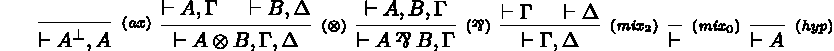
\includegraphics[width=0.75\linewidth,height=0.4\textheight,keepaspectratio]{graphic-03.pdf}\end{center}
 
% END S4.SS1.p2
 
% BEGIN S4.SS1.p3
 
The (hyp) rule introduces an hypothesis $A$ in a derivation, with $A$ a single formula. We restrict ourselves to a single formula not because we consider the ($\textnormal{{mix}}_{2}$) rule but because substitution of proof structures along more than one edge is much more complex. In this restricted setting, it is clear that all hypotheses formulas of a proof belong to distinct sequents and that we only need substitution of one hypothesis at a time. If $\pi$ is a derivation with hypotheses $\vdash A_{1}$, …, $\vdash A_{n}$ and conclusion $\vdash B_{1},\dotsc,B_{k}$, we call $\pi$ a derivation of $A_{1},\dotsc,A_{n}\vdash B_{1},\dotsc,B_{k}$. If $\pi_{1}$ is a derivation of $\Sigma\vdash\Gamma,A$ and $\pi_{2}$ is a derivation of $A,\Theta\vdash\Delta$, the substitution of $\pi_{1}$ in $\pi_{2}$ is a derivation of $\Sigma,\Theta\vdash\Gamma,\Delta$: it is obtained from $\pi_{2}$ by replacing the (hyp) rule on $\vdash A$ with $\pi_{1}$ (this adds $\Gamma$ to all sequents of $\pi_{2}$ below $\vdash A$).\par
 
% END S4.SS1.p3
 
% BEGIN S4.SS1.p4
 
To be formal, we should be more precise on how we handle occurrences of formulas (e.g. considering sequents as lists and having an explicit exchange rule) but we keep this implicit.\par
 
% END S4.SS1.p4
 
% BEGIN S4.SS1.p5
 
We also consider the following rewriting of derivations which we call mix-Rétoré reduction (due to its similarity to Rétoré’s reduction on the exponential connective $\wn$ [6, page 77], with contraction and weakening forming a monoid):\par
 
% END S4.SS1.p5
 
% BEGIN S4.SS1.p6
 
\begin{center}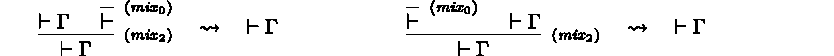
\includegraphics[width=0.75\linewidth,height=0.4\textheight,keepaspectratio]{graphic-04.pdf}\end{center}
 
% END S4.SS1.p6
 
% BEGIN S4.SS1.p7
 
It defines a confluent and strongly normalizing rewriting system on derivations.\par
 
% END S4.SS1.p7
 
% BEGIN Thmtheorem9
 
\par\medskip\noindent\textbf{Lemma 9 (Mix-Rétoré Normal Forms).}\par
 
% BEGIN Thmtheorem9.p1
 
If $\pi$ is a derivation in mix-Rétoré normal form, either it is 
\begin{center}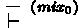
\includegraphics[width=0.75\linewidth,height=0.4\textheight,keepaspectratio]{graphic-05.pdf}\end{center}
 , or it does not contain the ($\textnormal{{mix}}_{0}$) rule and it proves a non-empty sequent.\par
 
% END Thmtheorem9.p1
 
% END Thmtheorem9
 
% END S4.SS1
 
% BEGIN S4.SS2
 
\par\medskip\noindent\textbf{4.2 Proof Structures}\par
 
% BEGIN S4.F5
   
% BEGIN S4.F5.fig1

\begin{center}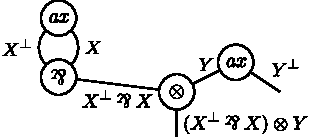
\includegraphics[width=0.75\linewidth,height=0.4\textheight,keepaspectratio]{graphic-06.pdf}\end{center}
 
Figure 4: Example of proof structure.\par
 
% END S4.F5.fig1
   
% BEGIN S4.F5.fig2

\begin{center}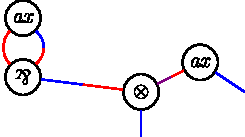
\includegraphics[width=0.75\linewidth,height=0.4\textheight,keepaspectratio]{graphic-07.pdf}\end{center}
 
Figure 5: Locally colored proof structure.\par
 
% END S4.F5.fig2
   
% END S4.F5
 
% BEGIN S4.SS2.p1
 
A proof structure is a partial graph with labeled vertices and edges. Edges are labeled with formulas, and vertices with names of the three following rules: ax, $\otimes$ or . Vertices are named according to their label: ax-vertices, $\otimes$-vertices and -vertices. Some additional local constraints are required depending on the label of vertices, also pictured below:\par
 
% END S4.SS2.p1
 
% BEGIN S4.SS2.p2
 
\begin{center}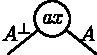
\includegraphics[width=0.75\linewidth,height=0.4\textheight,keepaspectratio]{graphic-08.pdf}\end{center}

\begin{center}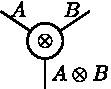
\includegraphics[width=0.75\linewidth,height=0.4\textheight,keepaspectratio]{graphic-09.pdf}\end{center}

\begin{center}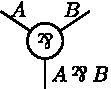
\includegraphics[width=0.75\linewidth,height=0.4\textheight,keepaspectratio]{graphic-10.pdf}\end{center}
 
\par
  
\par\noindent  $\blacksquare$ 
% BEGIN S4.I1.i1.p1
 
each ax-vertex has two incident edges, called its conclusions, labeled with dual formulas;\par
 
% END S4.I1.i1.p1
 
 
\par\noindent  $\blacksquare$ 
% BEGIN S4.I1.i2.p1
 
each $\otimes$-vertex has three incidents edges, labeled by $A$, $B$ and $A\otimes B$ for some formulas $A$ and $B$; the first two edges are its premises, the last one is its conclusion;\par
 
% END S4.I1.i2.p1
 
 
\par\noindent  $\blacksquare$ 
% BEGIN S4.I1.i3.p1
 
each -vertex has three incidents edges, labeled by $A$, $B$ and $A\invamp B$ for some formulas $A$ and $B$; the first two edges are its premises, the last one is its conclusion;\par
 
% END S4.I1.i3.p1
 
 
\par\noindent  $\blacksquare$ 
% BEGIN S4.I1.i4.p1
 
an edge is the premise of at most one vertex and the conclusion of at most one vertex.\par
 
% END S4.I1.i4.p1
 
  
% END S4.SS2.p2
 
% BEGIN S4.SS2.p3
 
An example of proof structure is given on Figure 5. A vertex is terminal when all its conclusions have exactly one endpoint (or equivalently, are not premises). An edge that is the premise of no vertex is a conclusion of the proof structure. An edge that is the conclusion of no vertex is an hypothesis of the proof structure.\par
 
% END S4.SS2.p3
 
% BEGIN Thmtheorem10
 
\par\medskip\noindent\textbf{$\blacktriangleright$ Remark 10.}\par
 
% BEGIN Thmtheorem10.p1
 
There are many ways to define proof structures. In the typed multiplicative case considered here, it is easy to check our definition is equivalent to others in the literature (e.g. [14, 32]). To strictly recover the usual notion of proof structure, and to distinguish for example the two proof structures with two conclusions typed $X^{\perp}\invamp X^{\perp}$ and $X\otimes X$, we should impose an order on the premises of vertices, as well as on the hypotheses and conclusions: we do not do so since this has no impact on correctness nor on (proofs of) sequentialization.\par
 
% END Thmtheorem10.p1
 
% END Thmtheorem10
 
% BEGIN S4.SS2.p4
 
To identify proof structures corresponding to proofs, and create a distinction between $\otimes$- and -vertices, it is usual to ask for a proof structure to respect a correctness criterion. As explained in the introduction, we use one due to Danos and Regnier [7]. A path in a proof structure is called switching when it does not contain the two premises of any -vertex. A proof structure is DR-correct (and is called a proof net) if it has no switching cycle.\par
 
% END S4.SS2.p4
 
% BEGIN Thmtheorem11
 
\par\medskip\noindent\textbf{$\blacktriangleright$ Remark 11.}\par
 
% BEGIN Thmtheorem11.p1
 
The original definition of the acyclicity condition in the Danos-Regnier correctness criterion [7] (extended to ($\textnormal{{mix}}_{2}$) in [11]) is in fact slightly different. They consider correctness graphs: graphs obtained by removing one of the two premises of each -vertex. A proof structure is correct when all its correctness graphs are acyclic (and connected in the original work without the mix rules). This condition is equivalent to the fact that any cycle in the proof structure must contain the two premises of some -vertex (i.e. no cycle is feasible in the sense of [11]). This is also equivalent to the apparently weaker condition that any cycle in the proof structure must go through the two premises of some -vertex consecutively:\par
 
% END Thmtheorem11.p1
 
% END Thmtheorem11
 
% BEGIN Thmtheorem12
 
\par\medskip\noindent\textbf{Lemma 12 (Local-Global Principle).}\par
 
% BEGIN Thmtheorem12.p1
 
A simple path that never goes through the two premises of a -vertex consecutively (including as last and first edges for a cycle) is a switching path.\par
 
% END Thmtheorem12.p1
 
% END Thmtheorem12
 
% END S4.SS2
 
% BEGIN S4.SS3
 
\par\medskip\noindent\textbf{4.3 Desequentialization}\par
 
% BEGIN S4.SS3.p1
 
We define, by induction on a derivation $\pi$ of $A_{1},\dotsc,A_{n}\vdash B_{1},\dotsc,B_{k}$, its desequentialization $\mathcal{D}(\pi)$ which is a DR-correct proof structure with hypotheses labeled $A_{1}$, …, $A_{n}$ and conclusions labeled $B_{1}$, …, $B_{k}$.\par
  
\par\noindent  $\blacksquare$ 
% BEGIN S4.I2.i1.p1
 
If $\pi$ is reduced to an (ax) rule with conclusion $\vdash A^{\perp},A$, then $\mathcal{D}(\pi)$ is the proof structure with one ax-vertex $v$ and two edges labeled $A^{\perp}$ and $A$, both with unique endpoint $v$.\par
  
\begin{center}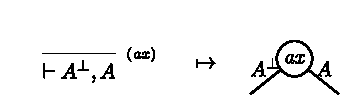
\includegraphics[width=0.75\linewidth,height=0.4\textheight,keepaspectratio]{graphic-11.pdf}\end{center}
  
% END S4.I2.i1.p1
 
 
\par\noindent  $\blacksquare$ 
% BEGIN S4.I2.i2.p1
 
If the last rule of $\pi$ is a ($\otimes$) rule applied to two derivations $\pi_{1}$ and $\pi_{2}$ then $\mathcal{D}(\pi)$ is obtained from the disjoint union of $\mathcal{D}(\pi_{1})$ and $\mathcal{D}(\pi_{2})$ by adding a new $\otimes$-vertex $v$. The conclusions of $\mathcal{D}(\pi_{1})$ and $\mathcal{D}(\pi_{2})$ labeled by the principal formulas $A$ and $B$ of the ($\otimes$) rule now have $v$ as an additional endpoint, and we add a new edge, labeled $A\otimes B$, with $v$ as unique endpoint.\par
  
\begin{center}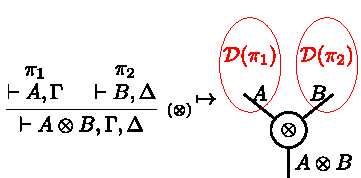
\includegraphics[width=0.75\linewidth,height=0.4\textheight,keepaspectratio]{graphic-12.pdf}\end{center}
  
% END S4.I2.i2.p1
 
 
\par\noindent  $\blacksquare$ 
% BEGIN S4.I2.i3.p1
 
If the last rule of $\pi$ is a () rule applied to a derivation $\pi_{1}$ then $\mathcal{D}(\pi)$ is obtained from $\mathcal{D}(\pi_{1})$ by adding a new -vertex $v$. The conclusions of $\mathcal{D}(\pi_{1})$ labeled by the principal formulas $A$ and $B$ of the () rule now have $v$ as an additional endpoint, and we add a new edge, labeled $A\invamp B$, whose unique endpoint is $v$.\par
  
\begin{center}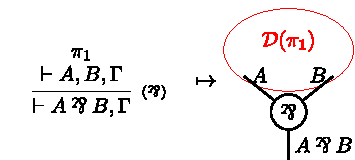
\includegraphics[width=0.75\linewidth,height=0.4\textheight,keepaspectratio]{graphic-13.pdf}\end{center}
  
% END S4.I2.i3.p1
 
 
\par\noindent  $\blacksquare$ 
% BEGIN S4.I2.i4.p1
 
If the last rule of $\pi$ is a ($\textnormal{{mix}}_{2}$) rule applied to two derivations $\pi_{1}$ and $\pi_{2}$ then $\mathcal{D}(\pi)$ is the disjoint union of $\mathcal{D}(\pi_{1})$ and $\mathcal{D}(\pi_{2})$.\par
  
\begin{center}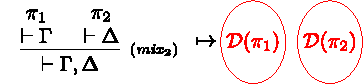
\includegraphics[width=0.75\linewidth,height=0.4\textheight,keepaspectratio]{graphic-14.pdf}\end{center}
  
% END S4.I2.i4.p1
 
 
\par\noindent  $\blacksquare$ 
% BEGIN S4.I2.i5.p1
 
If $\pi$ is reduced to a ($\textnormal{{mix}}_{0}$) rule, $\mathcal{D}(\pi)$ is the empty proof structure (no vertex, no edge).\par
  
\begin{center}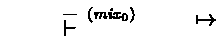
\includegraphics[width=0.75\linewidth,height=0.4\textheight,keepaspectratio]{graphic-15.pdf}\end{center}
  
% END S4.I2.i5.p1
 
 
\par\noindent  $\blacksquare$ 
% BEGIN S4.I2.i6.p1
 
If $\pi$ is reduced to a (hyp) rule on $\vdash A$, then $\mathcal{D}(\pi)$ is the proof structure with no vertex and a single edge with no endpoint, labeled $A$.\par
  
\begin{center}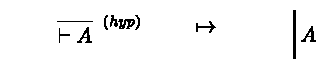
\includegraphics[width=0.75\linewidth,height=0.4\textheight,keepaspectratio]{graphic-16.pdf}\end{center}
  
% END S4.I2.i6.p1
 
  
There is a bijection between the (ax), ($\otimes$) and () rules of $\pi$ and the vertices of $\mathcal{D}(\pi)$. Moreover, if $\pi_{2}$ is obtained from $\pi_{1}$ by a mix-Rétoré reduction then $\mathcal{D}(\pi_{1})\simeq\mathcal{D}(\pi_{2})$.\par
 
% END S4.SS3.p1
 
% BEGIN Thmtheorem13
 
\par\medskip\noindent\textbf{Lemma 13 (Desequentialization of a substitution).}\par
 
% BEGIN Thmtheorem13.p1
 
If $\pi$ is the substitution of a derivation $\pi_{1}$ for a hypothesis $A$ in a derivation $\pi_{2}$, then $\mathcal{D}(\pi)$ is obtained from the disjoint union of $\mathcal{D}(\pi_{1})$ and $\mathcal{D}(\pi_{2})$ by identifying the conclusion $e$ of $\mathcal{D}(\pi_{1})$ labeled $A$ with the hypothesis $e^{\prime}$ of $\mathcal{D}(\pi_{2})$ labeled $A$. The obtained edge has label $A$ and endpoints the union of those of $e$ and $e^{\prime}$.\par
 
% END Thmtheorem13.p1
 
% END Thmtheorem13
 
% END S4.SS3
 
% END S4


% BEGIN S5
 
\par\medskip\noindent\textbf{5 Sequentialization from Parametrized Local Yeo}\par
 
% BEGIN S5.p1
 
This section is dedicated to show how sequentialization results (see [14, 7, 6, 11] for example) can be deduced from Theorem 8. We provide several proofs of the known statement:\par
 
% END S5.p1

% BEGIN S5.p2
 
The first step is to define the following local coloring c (see Figure 5 for an example):\par
  
\par\noindent  $\blacksquare$ 
% BEGIN S5.I1.i1.p1
 
for an ax-vertex $v$ of conclusions $e_{1}$ and $e_{2}$, set $\textnormal{{c}}(e_{1},v)=\text{{\color[rgb]{1,0,0}\definecolor[named]{%
pgfstrokecolor}{rgb}{1,0,0}solid}}$ and $\textnormal{{c}}(e_{2},v)=\text{{\color[rgb]{0,0,1}\definecolor[named]{%
pgfstrokecolor}{rgb}{0,0,1}dashed}}$;\par
 
% END S5.I1.i1.p1
 
 
\par\noindent  $\blacksquare$ 
% BEGIN S5.I1.i2.p1
 
for a $\otimes$-vertex $v$ of premises $e_{1}$ and $e_{2}$ and conclusion $f$, set $\textnormal{{c}}(e_{1},v)=\text{{\color[rgb]{1,0,0}\definecolor[named]{%
pgfstrokecolor}{rgb}{1,0,0}solid}}$, $\textnormal{{c}}(e_{2},v)=\text{{\color[rgb]{.5,0,.5}\definecolor[named]{%
pgfstrokecolor}{rgb}{.5,0,.5}dotted}}$ and $\textnormal{{c}}(f,v)=\text{{\color[rgb]{0,0,1}\definecolor[named]{%
pgfstrokecolor}{rgb}{0,0,1}dashed}}$;\par
 
% END S5.I1.i2.p1
 
 
\par\noindent  $\blacksquare$ 
% BEGIN S5.I1.i3.p1
 
for a -vertex $v$ of premises $e_{1}$ and $e_{2}$ and conclusion $f$, set $\textnormal{{c}}(e_{1},v)=\textnormal{{c}}(e_{2},v)=\text{{\color[rgb]{1,0,0}%
\definecolor[named]{pgfstrokecolor}{rgb}{1,0,0}solid}}$ and $\textnormal{{c}}(f,v)=\text{{\color[rgb]{0,0,1}\definecolor[named]{%
pgfstrokecolor}{rgb}{0,0,1}dashed}}$.\par
 
% END S5.I1.i3.p1
 
  
Note the cusp-points of a colored proof structure are exactly the pairs $(v,\text{{\color[rgb]{1,0,0}\definecolor[named]{pgfstrokecolor}{rgb}{1,0,0}%
solid}})$ where $v$ is a -vertex – which is in fact the only condition we need and requires a local coloring (see the left ax in Figure 5). In all this section, we assume proof structures to be colored this way. Then, the absence of switching cycles means there is no cusp-free cycle. Theorem 8 gives a splitting vertex for any set $P$ dominating cusp-points – i.e. pairs $(v,\text{{\color[rgb]{1,0,0}\definecolor[named]{pgfstrokecolor}{rgb}{1,0,0}%
solid}})$ with $v$ a -vertex.\par
 
% END S5.p2
 
% BEGIN S5.p3
 
Observe that, with the local coloring we have fixed, we recover the notions of splitting $\otimes$- or -vertex which play a crucial rôle in most of the sequentialization results for DR-correct proof structures: finding such a vertex allows to decompose a proof net in smaller components, and to deduce sequentialization inductively. Indeed, for $v$ a splitting vertex:\par
  
\par\noindent  $\blacksquare$ 
% BEGIN S5.I2.i1.p1
 
If $v$ is a $\otimes$-vertex with conclusion labeled $A\otimes B$, its premises and conclusion are not connected, except through $v$. By removing $v$, we obtain three disjoint proof structures: $\rho_{1}$ with a conclusion $A$, $\rho_{2}$ with a conclusion $B$, and $\rho_{0}$ with a hypothesis $A\otimes B$. By induction hypothesis, we get corresponding derivations $\pi_{1}$, $\pi_{2}$ and $\pi_{0}$. By adding a ($\otimes$) rule to $\pi_{1}$ and $\pi_{2}$, and substituting the obtained derivation in $\pi_{0}$, we get a sequentialization of $\rho$.\par
 
% END S5.I2.i1.p1
 
 
\par\noindent  $\blacksquare$ 
% BEGIN S5.I2.i2.p1
 
If $v$ is a -vertex with conclusion labeled $A\invamp B$, its premises are not connected to its conclusion, except through $v$. By removing $v$ from $\rho$, we obtain two disjoint proof structures: $\rho_{1}$ with conclusions $A$ and $B$, and $\rho_{0}$ with a hypothesis $A\invamp B$. By induction hypothesis, we get two corresponding derivations $\pi_{1}$ and $\pi_{0}$. By adding a () rule to $\pi_{1}$ and substituting the obtained derivation in $\pi_{0}$, we obtain a sequentialization of $\rho$.\par
 
% END S5.I2.i2.p1
 
 
\par\noindent  $\blacksquare$ 
% BEGIN S5.I2.i3.p1
 
If $v$ is an ax-vertex with conclusions labeled $A^{\perp}$ and $A$, its conclusions are not connected, except through $v$. By removing $v$ from $\rho$, we obtain two disjoint proof structures: $\rho_{1}$ with a hypothesis $A^{\perp}$ and $\rho_{2}$ with a hypothesis $A$. By induction hypothesis, we get two corresponding derivations $\pi_{1}$ and $\pi_{2}$. By first substituting a derivation reduced to a single (ax) rule into $\pi_{1}$, and then substituting the result in $\pi_{2}$, we get a sequentialization of $\rho$.\par
 
% END S5.I2.i3.p1
 
  
% END S5.p3
 
% BEGIN S5.p4
 
We fix a DR-correct proof structure $\rho$: $\rho$ has no cusp-free cycle. We review how natural choices for the parameter $P$ in Theorem 8 yield various proofs of Theorem 14, differing only in the order in which splitting vertices are selected along the sequentialization procedure. Each of these choices satisfies the hypothesis of Theorem 8 trivially: $P$ contains all cusp-points.\par
  General splitting vertices.  
% BEGIN S5.I3.ix1.p1
 
Take $P$ the set of all vertex-color pairs. By Theorem 8, for each $\lhd$-maximal element $(v,\alpha)\in P$, the vertex $v$ is splitting. As described above, $v$ allows to decompose $\rho$ and to go on by induction. It remains only to treat the case $P=\emptyset$, i.e. without vertex. If $\rho$ is empty (no vertex, no edge), it is the desequentialization of the derivation reduced to a ($\textnormal{{mix}}_{0}$) rule. If $\rho$ is a single edge (with no endpoint), it is the desequentialization of a derivation reduced to a (hyp) rule. Else, decomposing $\rho$ into connected components corresponds to applying ($\textnormal{{mix}}_{2}$) rules on the sequent calculus side.\par
 
% END S5.I3.ix1.p1
  Splitting - or $\otimes$-vertices.  
% BEGIN S5.I3.ix2.p1
 
Let $P\coloneqq\{(v,\alpha)\mid\text{$v$ is a $\otimes$- or $\invamp$-vertex and $%
\alpha$ is a color in $\rho$}\}$. By Theorem 8, each $\lhd$-maximal element $(v,\alpha)\in P$ yields a splitting vertex $v$, which must be a - or $\otimes$-vertex. We reason inductively as before, which leaves only the case $P=\emptyset$: all vertices must be ax-vertices and we reason as above, splitting along connected components that can be an ax-vertex with its two conclusions or an edge without endpoint.\par
 
% END S5.I3.ix2.p1
  Splitting -vertices (a.k.a. sections) [7].  
% BEGIN S5.I3.ix3.p1
 
Let $P$ be the set of all cusp-points: a $\lhd$-maximal element of $P$ is $(v,\alpha)$ with $v$ a splitting -vertex by Theorem 8, so we can reason inductively. It remains only to treat the case $P=\emptyset$ (i.e. no -vertex, hence no cusp in $\rho$): by DR-correctness, $\rho$ is cycle-free, and all the remaining vertices are splitting.\par
 
% END S5.I3.ix3.p1
  Splitting terminal vertices [14].  
% BEGIN S5.I3.ix4.p1
 
Let $P\coloneqq\{(v,\text{{\color[rgb]{1,0,0}\definecolor[named]{pgfstrokecolor}{%
rgb}{1,0,0}solid}})\mid\text{$v$ is a $\otimes$- or $\invamp$-vertex}\}\cup\{(%
v,\text{{\color[rgb]{.5,0,.5}\definecolor[named]{pgfstrokecolor}{rgb}{.5,0,.5}%
dotted}})\mid\text{$v$ is a $\otimes$-vertex}\}$, and let $(v,\alpha)\in P$ be maximal for $\lhd$. Then $v$ is not only splitting by Theorem 8, but it is also terminal. Indeed, otherwise its conclusion $e$ has another endpoint $u$. This $u$ must be a $\otimes$- or -vertex (as $e$ can only be one of its premises, and these are the only vertices with premises). Then $(v,\alpha)\overset{(v,e,u)}{\Rsh}(u,\textnormal{{c}}(e,u))$ since $\textnormal{{c}}(e,v)=\text{{\color[rgb]{0,0,1}\definecolor[named]{%
pgfstrokecolor}{rgb}{0,0,1}dashed}}\neq\alpha$. Moreover, we cannot have $(u,\textnormal{{c}}(e,u))\overset{p}{\Rsh}(v,\beta)$ for a color $\beta$ as this would yield a cusp-free cycle $(v,e,u)\cdot p$. We obtain $(v,\alpha)\lhd(u,\textnormal{{c}}(e,u))$, contradicting the maximality of $(v,\alpha)$. So, if $P\neq\emptyset$, we obtain a splitting terminal $\otimes$- or -vertex. The sequentialization procedure is then the same as before, except that we can focus on terminal vertices all along.\par
 
% END S5.I3.ix4.p1
   
% END S5.p4

% BEGIN Thmtheorem14
 
\par\medskip\noindent\textbf{Theorem 14 (Sequentialization [14, 7, 6, 11]).}\par
 
% BEGIN Thmtheorem14.p1
 
Given a DR-correct proof structure $\rho$, there exists a derivation $\pi$ in $\textnormal{{MLL}}^{0,2}_{\textnormal{{hyp}}}$ such that $\rho\simeq\mathcal{D}(\pi)$; $\pi$ is called a sequentialization of $\rho$.\par
 
% END Thmtheorem14.p1
 
% END Thmtheorem14

\begin{thebibliography}{99}

% BEGIN bib
 
\par\medskip\noindent\textbf{References}\par
  
\par\noindent  [1]  A. Abouelaoualim, K.Ch. Das, L. Faria, Y. Manoussakis, C. Martinhon, and R. Saad.  Paths and trails in edge-colored graphs.  Theoretical Computer Science, 409(3):497–510, 2008.  doi:10.1016/j.tcs.2008.09.021.  
 
\par\noindent  [2]  Adrian Bondy and U. S. R. Murty.  Graph Theory.  Number 1 in Graduate Texts in Mathematics. Springer London, 2008.  URL: https://link.springer.com/book/9781846289699.  
 
\par\noindent  [3]  Jørgen Bang-Jensen and Gregory Z Gutin.  Digraphs: theory, algorithms and applications.  Springer Science \& Business Media, 2008.  
 
\par\noindent  [4]  Claude Berge.  Two theorems in graph theory.  Proceedings of the National Academy of Sciences of the United States of America, 43(9):842–844, September 1957.  URL: https://www.jstor.org/stable/89875.  
 
\par\noindent  [5]  Pierre-Louis Curien.  Introduction to linear logic and ludics, part II.  lecture notes cs/0501039, arXiv, 2005.  URL: https://arxiv.org/abs/cs/0501039.  
 
\par\noindent  [6]  Vincent Danos.  La Logique Linéaire appliquée à l’étude de divers processus de normalisation (principalement du $\lambda$-calcul).  Thèse de doctorat, Université Paris VII, 1990.  
 
\par\noindent  [7]  Vincent Danos and Laurent Regnier.  The structure of multiplicatives.  Archive for Mathematical Logic, 28:181–203, 1989.  doi:10.1007/BF01622878.  
 
\par\noindent  [8]  Paulin Jacobé de Naurois and Virgile Mogbil.  Correctness of linear logic proof structures is NL-complete.  Theoretical Computer Science, 412(20):1941–1957, 2011.  doi:10.1016/J.TCS.2010.12.020.  
 
\par\noindent  [9]  Rémi Di Guardia.  Identity of Proofs and Formulas using Proof-Nets in Multiplicative-Additive Linear Logic.  Thèse de doctorat, École Normale Supérieure de Lyon, September 2024.  
 
\par\noindent  [10]  Thomas Ehrhard.  A new correctness criterion for MLL proof nets.  In Thomas A. Henzinger and Dale Miller, editors, Joint Meeting of the Twenty-Third EACSL Annual Conference on Computer Science Logic (CSL) and the Twenty-Ninth Annual ACM/IEEE Symposium on Logic in Computer Science (LICS), pages 38:1–38:10. ACM, 2014.  doi:10.1145/2603088.2603125.  
 
\par\noindent  [11]  Arnaud Fleury and Christian Retoré.  The mix rule.  Mathematical Structures in Computer Science, 4(2):273–285, 1994.  doi:10.1017/S0960129500000451.  
 
\par\noindent  [12]  Shinya Fujita, Ruonan Li, and Shenggui Zhang.  Color degree and monochromatic degree conditions for short properly colored cycles in edge-colored graphs.  Journal of Graph Theory, 87(3):362–373, 2018.  doi:10.1002/jgt.22163.  
 
\par\noindent  [13]  Hortensia Galeana-Sánchez, Rocío Rojas-Monroy, Rocío Sánchez-López, and Juana Imelda Villareal-Valdés.  H-cycles in H-colored multigraphs.  Graphs and Combinatorics, 38:62, 2022.  doi:10.1007/s00373-022-02464-4.  
 
\par\noindent  [14]  Jean-Yves Girard.  Linear logic.  Theoretical Computer Science, 50:1–102, 1987.  doi:10.1016/0304-3975(87)90045-4.  
 
\par\noindent  [15]  Jean-Yves Girard.  Geometry of interaction I: an interpretation of system ${F}$.  In Ferro, Bonotto, Valentini, and Zanardo, editors, Logic Colloquium ’88. North-Holland, 1988.  
 
\par\noindent  [16]  Jean-Yves Girard.  Quantifiers in linear logic II.  In Corsi and Sambin, editors, Nuovi problemi della logica e della filosofia della scienza, pages 79–90, Bologna, 1991. CLUEB.  
 
\par\noindent  [17]  Jean-Yves Girard.  Linear logic: its syntax and semantics.  In Jean-Yves Girard, Yves Lafont, and Laurent Regnier, editors, Advances in Linear Logic, volume 222 of London Mathematical Society Lecture Note Series, pages 1–42. Cambridge University Press, 1995.  
 
\par\noindent  [18]  Jean-Yves Girard.  Proof-nets: the parallel syntax for proof-theory.  In Aldo Ursini and Paolo Agliano, editors, Logic and Algebra, volume 180 of Lecture Notes In Pure and Applied Mathematics, pages 97–124, New York, 1996. Marcel Dekker.  
 
\par\noindent  [19]  Jerrold W. Grossman and Roland Häggkvist.  Alternating cycles in edge-partitioned graphs.  Journal of Combinatorial Theory, Series B, 34(1):77–81, 1983.  doi:10.1016/0095-8956(83)90008-4.  
 
\par\noindent  [20]  Giulio Guerrieri, Giulia Manara, Lorenzo Tortora de Falco, and Lionel Vaux Auclair.  Confluence for proof-nets via parallel cut elimination.  In Nikolaj S. Bjørner, Marijn Heule, and Andrei Voronkov, editors, LPAR 2024: Proceedings of 25th Conference on Logic for Programming, Artificial Intelligence and Reasoning, Port Louis, Mauritius, May 26-31, 2024, volume 100 of EPiC Series in Computing, pages 464–483. EasyChair, 2024.  doi:10.29007/VKFN.  
 
\par\noindent  [21]  Stefano Guerrini.  Correctness of multiplicative proof nets is linear.  In Proceedings of the fourteenth annual symposium on Logic In Computer Science, pages 454–463, Trento, July 1999. IEEE, IEEE Computer Society Press.  doi:10.1109/LICS.1999.782640.  
 
\par\noindent  [22]  Dominic Hughes.  Simple multiplicative proof nets with units, 2005.  arXiv:math/0507003.  
 
\par\noindent  [23]  Dominic Hughes.  Simple free star-autonomous categories and full coherence.  Journal of Pure and Applied Algebra, 216(11):2386–2410, 2012.  doi:10.1016/j.jpaa.2012.03.020.  
 
\par\noindent  [24]  Dominic Hughes and Rob van Glabbeek.  Proof nets for unit-free multiplicative-additive linear logic.  ACM Transactions on Computational Logic, 6(4):784–842, 2005.  doi:10.1145/1094622.1094629.  
 
\par\noindent  [25]  Anton Kotzig.  On the theory of finite graphs with a linear factor II.  Matematicko-Fyzikálny Časopis, 09(3):136–159, 1959.  In Slovak, with as original title Z teórie konečných grafov s lineárnym faktorom II.  URL: https://eudml.org/doc/29908.  
 
\par\noindent  [26]  Yves Lafont.  From proof nets to interaction nets.  In Jean-Yves Girard, Yves Lafont, and Laurent Regnier, editors, Advances in Linear Logic, volume 222 of London Mathematical Society Lecture Note Series, pages 225–247. Cambridge University Press, 1995.  
 
\par\noindent  [27]  Olivier Laurent.  Polynomial time in untyped elementary linear logic.  Theoretical Computer Science, 813:117–142, 2020.  doi:10.1016/J.TCS.2019.10.002.  
 
\par\noindent  [28]  Ruonan Li and Bo Ning.  A revisit to Bang-Jensen-Gutin conjecture and Yeo’s theorem.  preprint, 2022.  doi:10.48550/arXiv.2207.03793.  
 
\par\noindent  [29]  Paul-André Melliès.  A topological correctness criterion for multiplicative non-commutative logic.  In Thomas Ehrhard, Jean-Yves Girard, Paul Ruet, and Philip J. Scott, editors, Linear Logic in Computer Science, volume 316 of London Mathematical Society Lecture Note Series, pages 283–322. Cambridge University Press, November 2004.  
 
\par\noindent  [30]  François Métayer.  Homology of proof-nets.  Archive for Mathematical Logic, 33(3):169–188, 1994.  doi:10.1007/bf01203031.  
 
\par\noindent  [31]  Gleb Nenashev.  A short proof of Kotzig’s theorem.  preprint, 2014.  doi:10.48550/arXiv.1402.0949.  
 
\par\noindent  [32]  Lê Thành Dũng Nguy$\tilde{\hat{\text{e}}}$n.  Unique perfect matchings, forbidden transitions and proof nets for linear logic with mix.  Logical Methods in Computer Science, 16(1), February 2020.  doi:10.23638/LMCS-16(1:27)2020.  
 
\par\noindent  [33]  Michele Pagani and Lorenzo Tortora de Falco.  Strong normalization property for second order linear logic.  Theoretical Computer Science, 411(2):410–444, 2010.  doi:10.1016/J.TCS.2009.07.053.  
 
\par\noindent  [34]  Christian Retoré.  Handsome proof-nets: perfect matchings and cographs.  Theoretical Computer Science, 294(3):473–488, 2003.  doi:10.1016/S0304-3975(01)00175-X.  
 
\par\noindent  [35]  Paul D. Seymour.  Sums of circuits.  Graph Theory and Related Topics, pages 341–355, 1978.  
 
\par\noindent  [36]  D. J. Shoesmith and T. J. Smiley.  Multiple-Conclusion Logic.  Cambridge University Press, 1978.  
 
\par\noindent  [37]  D. J. Shoesmith and T. J. Smiley.  Theorem on directed graphs, applicable to logic.  Journal of Graph Theory, 3(4):401–406, 1979.  doi:10.1002/jgt.3190030412.  
 
\par\noindent  [38]  Stefan Szeider.  On theorems equivalent with Kotzig’s result on graphs with unique 1-factors.  Ars Combinatoria, 73:53–64, 2004.  URL: https://www.ac.tuwien.ac.at/files/pub/szeider-AC-2004.pdf.  
 
\par\noindent  [39]  Anders Yeo.  A note on alternating cycles in edge-coloured graphs.  Journal of Combinatorial Theory, Series B, 69(2):222–225, 1997.  doi:10.1006/jctb.1997.1728.  
  
% END bib
\end{thebibliography}
\end{document}
